\documentclass{article}
\usepackage[utf8]{inputenc} % allows for non-ASCII characters
\usepackage[x11names]{xcolor}    % Color extensions
\usepackage[margin=1in]{geometry} % Formatting on page
\usepackage{array} % big arrays
\usepackage{amsmath} % Math symbols
\usepackage{amsthm}   
\usepackage{amssymb}
\usepackage[backend=bibtex]{biblatex} % bibliography
\usepackage{bm} % bold for greek letters
\usepackage{cancel}
\usepackage[format=hang]{caption}
\usepackage{enumitem} % Enumerating things
\usepackage{esint} % better double and triple Integrals
\usepackage{etoc}
\usepackage{fancyhdr} % Headers
    \pagestyle{fancy}
\usepackage{float}
\usepackage{gensymb}
\usepackage{physics} % easier commands for physics things
\usepackage{relsize}  % allows for larger/smaller math 
\usepackage{textcomp} % Gets rid of perthousand error
\usepackage{upquote}  % fixes quotes in verbatim environment
\usepackage{verbatim} % Allows for comment environment
\usepackage{tikz} % pictures
	\usetikzlibrary{calc}
	\usetikzlibrary{decorations.markings}
	\usetikzlibrary{3d}
	\usetikzlibrary{intersections}
\usepackage{pgfplots} % plots and graphics
	\pgfplotsset{compat=newest} % or use compat=1.6
	\usepgfplotslibrary{fillbetween}
\usepackage{graphicx} % plots and graphics
\usepackage{wrapfig}
\usepackage{xparse} % Better commands
\usepackage[hidelinks]{hyperref}% References--THIS GOES LAST

% Packages that this breaks without: amsmath, gensymb, physics, hyperref, xcolor, xparse, and possibly others
\numberwithin{equation}{section} % amsmath command that renews equation counter in each section\
\def\ints{\int_\mathcal{S}} % Surface integral
\def\intv{\int_\mathcal{V}} % Volume integral with V subscript
\def\intall{\int_{-\infty}^{\infty}} % Integral over all space
\def\iintall{\iint_{\rm All Space}} % Integral over all space
\def\iiintall{\iiint_{\rm All Space}} % Integral over all space
\def\ik{4\pi\epsilon_0} % Inverse k for EM
\def\lap{\mathcal{L}}
\def\answerline{ % double horizontal line placed 0.5 cm below text, space between lines is 0.07 cm, then 0.75 cm of space 
	\vspace{0.5 cm}
	\hrule
	\vspace{0.07 cm}
	\hrule
	\vspace{0.75 cm}\noindent} % don't indent text after the line
\NewDocumentCommand\length{O{3pt}}{\setlength\jot{#1}} % for align vertical spacing, there's probably a better way to do this locally
\NewDocumentCommand\ft{s O{n} O{L}}{ % I dont want to write \sin(stuff) \cos(stuff) every time in fourier transforms (ft)
    \IfBooleanTF{#1}{
        \sin(\frac{#2 \pi}{#3}x)
    }{
        \cos(\frac{#2 \pi}{#3}x)
    }
}

\NewDocumentCommand\dl{s}{\IfBooleanTF{#1}{}{\cdot} d\mathbf{l}} % quicker curve integral dl, if no star, it also makes the dot 
\NewDocumentCommand\da{s}{\IfBooleanTF{#1}{}{\cdot} d\mathbf{a}} % quicker surface integral da, if no star, it also makes the dot 
\NewDocumentCommand\oo{O{1} m} {\frac{#1}{#2}}   % reciprocal- 'one over', option to make it a regular fraction because oo is still quicker to type.
\NewDocumentCommand\thetitle{m O{}}{ \title{ \hypertarget{top}{\textbf{#1}} \\ \large {#2} } } %Bold title that is a hypertarget, optional bolded subtitle that's scaled properly 

\NewDocumentCommand \e {s m}{ % basis vector command
	\IfBooleanTF{#1} % \e{x} for x hat notation, \e*{x} for e_x notation
	{\mathbf{\hat{e}_{#2}}}
	{\bm{\hat{#2}}}} % from package bm, more powerful than \mathbf} 
\NewDocumentCommand \parametric {m}{ %command for getting boundary conditions with a "{" on the left
    \left\{ 
	\begin{gathered}
		\begin{matrix}
			#1
    		\end{matrix}
	\end{gathered}
	 \right.}
\NewDocumentCommand \der {s O{} m g}{ % custom derivative command
     \IfBooleanTF{#1} % if \der*, #1 is true, euler notation used, if \der , #1 is false, d/dx is used 
    {\IfNoValueTF{#4}  % g returns -NoValue- if no argument (read below)
        {\mathrm{D}_{#3}^{#2}}  % g is included so \der{x} and \der{f}{x} both have x in the denominator
        {\mathrm{D}_{#4}^{#2}#3}
            }
    {\IfNoValueTF{#4}
        {\frac{\mathrm{d}^{#2}}{\mathrm{d} #3^{#2}}}
        {\frac{\mathrm{d}^{#2} #3}{\mathrm{d} #4^{#2}}}
	}}    
\NewDocumentCommand \pder {s O{} m g}{ % custom partial derivative command, allows for euler notation if starred
     \IfBooleanTF{#1}
        {\IfNoValueTF{#4}
            {\partial_{#3}^{#2}}
            {\partial_{#4}^{#2}#3}
                }
        {\IfNoValueTF{#4}
            {\frac{\partial^{#2}}{\partial #3^{#2}}}
            {\frac{\partial^{#2} #3}{\partial #4^{#2}}}
                }} 
                
\NewDocumentCommand \header {m m m}{
	\fancyhead[L]{#1} 
	\fancyhead[C]{\hyperlink{top}{ \textbf{#2} }}
	\fancyhead[R]{#3}
	\fancyfoot[C]{--\thepage--}
	\pagestyle{fancy}
	\setlength\headheight{17pt}}
    
\NewDocumentCommand{\coloredanswer}{O{LavenderBlush2} m}{ % makes coloredbox with pretty color
	\mathchoice
	{\colorbox{#1}{$\displaystyle #2$}}
	{\colorbox{#1}{$\textstyle #2$}}
	{}
	{}}

\newcounter{probcount} % new counter for problem numbers, starts at 0 by default
\NewDocumentEnvironment{ problem } {O{} +b} %Problem environment for homework, autocounts numbers, behaves like a section and can get listed (and hyperlinked) in the toc. 
	{\addtocounter{probcount}{1} % increase counter at the beginning of every problem
	 \phantomsection % invisible page marker for hyperref
	 \addcontentsline{toc}{subsection}{Problem \theprobcount. {\it#1}} % add "Problem \theprobcount. \textit{#1}" to table of contents (toc) as if it were a subsection
	 \begin{trivlist} % begin unmarked ("trivial") list
	 \item {\bf Problem \theprobcount.} {\it#1} % print Problem with the counter and optional text 
	 \item #2  % +b is for inputs that are long
	 \end{trivlist} % end list
	}{} % don't do anything then "problem" environment ends, irrelevant because trivlist is already ended
	
\def\UM{\colorbox{blue}{\textcolor{Gold1}{\textbf{University of Michigan}}}} % School Pride
\def\EC{\href{https://github.com/CarpenterEvan/PhysicsReview}{\(\mathbb{E}\textsc{van}~\mathbb{C}\textsc{arpenter}\)}}
\endinput
\header{Physics 406}{$\uparrow\uparrow\uparrow$}{Evan Carpenter}
\thetitle{Physics 406 Homework}[Winter Semester 2022]
\date{}
\author{\EC}
\counterwithin{probcount}{section} % reset problem every section.
\addtolength{\jot}{0.25cm} % changes row spacing to 0.25cm in align environment. Equivalent to replacing all \\ with \\[0.25cm] in align environment. 
\def\dbar{{\mathchar'26\mkern-12mu d}} % found online
\NewDocumentCommand{\ten}{m O{}}{\times10^{#1}\text{#2}}
\NewDocumentCommand{\DerivCrush}{s m m m g}{
    \IfNoValueTF{#5}
        {   \IfBooleanTF{#1}
                {\frac{-\pder{#4}{#3}[#2]}{\pder{#4}{#2}[#3]}}
                {\oo{\pder{#3}{#2}[#4]}}
        }
        {\frac{\pder{#2}{#5}[#4]}{\pder{#3}{#5}[#4]}}
} % \DerivCrush{x}{y}{z} D1  \DerivCrush*{x}{y}{z} D2  \DerivCrush{x}{y}{z}{w} D3 
\NewDocumentCommand{\CrushStep}{m O{}}{~~\xrightarrow[#2]{~~#1~~}~~}
\begin{document}
\pagenumbering{gobble}
\maketitle
\tableofcontents
\newpage\pagenumbering{arabic}
\section{Homework 1}
    \begin{problem}
        Prove that the quantity $\displaystyle S=-k\sum_{r=1}^{n}p_r\ln(p_r)$ is a maximum when $p_r=\oo{n}$. You may need to use the inequality: $$\ln(\oo{np_r})\leq\qty(\oo{np_r}-1)$$
        This completes the proof that the choice of equal relative probabilities for the states in a microcanonical ensemble maximizes missing information (entropy).
        \answerline
    \end{problem}\newpage
    \begin{problem}[Reif 2.3]
        Consider an ensemble of classical 1-D Harmonic oscillators. 
        \begin{enumerate}[label=(\alph*)]
            \item Let the displacement $x$ of an oscillattor as a function of time $t$ be given by $x=A\cos(\omega t+\varphi)$. Assume that the phase angle $\varphi$ is equally likely to assume any value $0<\varphi<2\pi$. The probability $w(\varphi)d\varphi$ that $\varphi$ lies in the range between $\varphi,\varphi+d\varphi$ is then simply $$w(\varphi)d\varphi=\frac{d\varphi}{2\pi}$$For any fixed time $t$, find the probability $P(x)dx$ that $x$ lies between $x+dx$ by summing $w(\varphi)d\varphi$ over all angles for which $x$ lies in this range. Express $P(x)$ in terms of $A,x$. 
            \item Consider the classical phase space for such an ensemble of oscillators, their energy being known to lie in the small range between $E,E+\delta E$. Calculate $P(x)$ by taking the ratio of that volume of phase space lying in this energy range \emph{and} in the range between $x,x+dx$ to the total volume of phase space lying in the energy range between $E,E+\delta E$. Express $P(x)$ in terms of $E,x$. By relating $E$ to the amplitude $A$, show that the result is the same as that obtained in (a)
        \end{enumerate}
        \answerline
    \end{problem}\newpage
    \begin{problem}
        Consider an assembly of $N$ weakly interacting one dimensional harmonic oscillators, each with a mass $m$ and frequency $\omega$.
        \begin{enumerate}[label=(\alph*)]
            \item Describe the region of phase space that is accessible to this system
            if its energy lies between $E$ and $E + \delta E$.
            \item Use phase space considerations to find how entropy of this system depends on $E$. (There will be an additive constant independent of $E$ which you need not determine.)
            \item How would a microstate of this system be described in quantum mechanical terms?
        \end{enumerate}
        \answerline
        \textcolor{red}{What does weakly interacting mean? How do we define it, interacting with the system? not each other?}
    \end{problem}\newpage
    \begin{problem}
        Suppose that a particle moving in one dimension is confined to $x>0$, and it's energy is $E=\frac{p^2}{2m}+mgx$ Make a sketch to indicate what
        region of classical phase space is accessible to this particle if its energy lies between $E_0$ and $E_0+\delta E_0$.
        \begin{figure}[H]
            \centering
            \begin{tikzpicture}
                \begin{axis}[ultra thick,
                            samples=40,
                            range=0:2,
                            xtick={0},
                            ytick={0},
                            xticklabels={0,},
                            yticklabels={0,},
                            xlabel={Momentum $(p)$},
                            ylabel={Position $(x)$}]
                    \addplot [name path=E, blue, domain=-1:1]{-x^2+1} node [pos=0.25, anchor=west] {$E$};
                    \addplot [name path=dE, red, domain=-1.41:1.41]{-x^2+2} node [pos=0.25, anchor=east] {$E+dE$};
                    \addplot[thin, black, domain=-1.5:1.5]{0};
                    \addplot [purple!30] fill between [of = E and dE, soft clip={domain=-1.5:1.5}];
                \end{axis}
            \end{tikzpicture}
            \caption{Particle constrained between blue and red curves.}
        \end{figure}
    \end{problem}\newpage
\section{Homework 2}
    \begin{problem}
        \begin{enumerate}[label=(\alph*)]
            \item Show that the number of states $\phi(E)$ with energy less than $E$, for a particle of mass $m$ in a cubical box of side $L$ is:
            $$\phi(E)=\frac{\pi}{6}\qty(\frac{L}{\pi\hbar})^3\qty(2mE)^{3/2}$$
            Hint: Use the energy levels 2.1.3 in Reif and treat the n as continuous variables.
            \\[0.5 cm]
            Reif 2.1.3: $\displaystyle E=\frac{(\hbar \pi)^2}{2m}\qty[\qty(\frac{n_x}{L_x})^2+ \qty(\frac{n_y}{L_y})^2+ \qty(\frac{n_z}{L_z})^2]$
            \item Calculate $\Omega(E)$
            \item A nitrogen molecule at room temperature has a typical energy of $6\times10^{-14}$ergs. Calculate $\phi(E)$ for a particle in a box of side length 10cm. Also calculate $\Omega(E)$ assuming $\delta E=10^{-24}$ergs
        \end{enumerate}
        \answerline
        \begin{enumerate}[label=\alph*)]
            \item Reif 2.1.3 can be simplified, knowing that the box is a cube implies that $L_x=L_y=L_z\equiv L$. 
            \\
            The remaining $n_x,n_y,n_z$ describe a sphere of radius $R=n_x^2+n_y^2+n_z^2$ in phase space. 
            \begin{figure}[H]
                \centering
                \begin{tikzpicture}
                    \draw[-latex] (0,0,0)--(2,0,0) node [anchor=west]{$n_y$};
                    \draw[-latex] (0,0,0)--(0,2,0) node [anchor=south]{$n_z$};
                    \draw[-latex] (0,0,0)--(0,0,2) node [anchor=north east]{$n_x$};
                    \draw [thick, red] (0,0,0)--(0.7,0,0.7) node [anchor=north west]{R};
                    \begin{scope}[thick]
                        \draw[canvas is xz plane at y=0] (0,0)++(1,0) arc[start angle=0, end angle=90,radius=1];
                        \draw[canvas is xz plane at y=0.25] (0,0)++(0.96,0) arc[start angle=0, end angle=90,radius=0.96];
                        \draw[canvas is xz plane at y=0.5] (0,0)++(0.87,0) arc[start angle=0, end angle=90,radius=0.87];
                        \draw[canvas is xz plane at y=0.75] (0,0)++(0.68,0) arc[start angle=0, end angle=90,radius=0.68];
                        \draw[canvas is yz plane at x=0] (0,0)++(1,0) arc[start angle=0, end angle=90,radius=1];
                        \draw[canvas is xy plane at z=0] (0,0)++(1,0) arc[start angle=0, end angle=90,radius=1];
                    \end{scope}
                \end{tikzpicture}
                \caption*{$\displaystyle E=\frac{(\hbar \pi)^2}{2mL^2}\qty[\textcolor{Red1}{ n_x^2+ n_y^2+ n_z^2}]$}
            \end{figure} 
            All possible states for the system are contained in this sphere. Since we can assume $n_x,n_y,n_z$ are continuous, $\phi(E)$ is just the volume of this slice of the sphere ($V=\oo{8}\frac{4}{3}\pi R^3$): 
            \begin{equation*}
                \boxed{\phi(E)=\oo{8}\frac{4}{3}\pi R^3}\longrightarrow
                \boxed{\phi(E)=\oo[\pi]{6}\qty(\sqrt{2mE}\frac{L}{\hbar\pi})^3}
                \longrightarrow
                \boxed{\phi(E)=\frac{\pi}{6}\qty(\frac{L}{\pi\hbar})^3\qty(2mE)^{3/2}}\quad\checkmark
            \end{equation*}
            \item $\displaystyle \Omega(E)=\phi(E+\delta E)-\phi(E)=\frac{\phi(E+\delta E)-\phi(E)}{\delta E}\delta E= \der{\phi}{E}\delta E$
            \begin{align*}
                \Omega(E)&=\der{\phi}{E}\delta E=\frac{\pi}{6}\qty(\frac{L}{\pi\hbar})^3\qty(\frac{3}{\cancel{2}})(\cancel{2}m)\qty(2mE)^{1/2}\delta E
                \\
                &\coloredanswer{\Omega(E)=\frac{m\pi}{2}\sqrt{2mE}\qty(\frac{L}{\pi\hbar})^3\delta E}
            \end{align*}
            \item \textcolor{Red1}{Find energy in joules, plug in to phi equation with other units, or just use cgs}
        \end{enumerate}
    \end{problem}\newpage
    \begin{problem}[Reif 2.4]
        Consider an isolated system consisting of a large number $N$ of weakly interacting localized particles of spin $\frac{1}{2}$. Each particle has a magnetic moment $\mu$ which can point either parallel or antiparallel to an applied field $H$. The energy of the system is then $E=-(n_1-n_2)\mu H$, where $n_1$ is the number of spins aligned parallel to $H$ and $n_2$ is the number of spins aligned antiparallel to $H$. 
        \begin{enumerate}[label=(\alph*)]
            \item Consider the energy range between $E+\delta E$ where $\delta E$ is much smaller than $E$, but $E$ is still microscopically large, so $\mu H \ll \delta E\ll E$. What is $\Omega(E)$ (the total number of states  in the energy range)?
            \item Write down an expression for $\ln(\Omega(E))$ as a function of $E$. Simplify this expression by using Stirling's formula in it's simplest form: $$\ln(n!)\approx n\ln(n)-n$$
            \item Assume that the energy $E$ is in a region where $\Omega(E)$ is appreciable~$\rightarrow$~that it is not close to the extreme possible values $\pm N\mu H$ which it can assume. In this case apply a Gaussian approximation to part (a) to obtain a simple expression for $\Omega(E)$ as a function of $E$.
        \end{enumerate}
        \answerline
        \begin{enumerate}[label=\alph*)]
            \item Using the equation $E=-(n_1-n_2)\mu H$ and knowing that \begin{equation*}
                \Omega(E)=~_NC_{n_1}\delta E=\frac{N!}{n_1!(N-n_1)!}=\frac{N!}{n_1!n_2!}\delta E
            \end{equation*}
            \begin{align*}
                E&=-(n_1-n_2)\mu H=-(n_1-(N-n_1))\mu H=-(2n_1-N)\mu H
                \\
                &\boxed{n_1=\frac{N}{2}-\frac{E}{2\mu H}\quad,\quad n_2=\frac{N}{2}+\frac{E}{2\mu H}}
                \\
                \delta E&=|-2\delta n\mu H|
                \\
                &\coloredanswer{\Omega(E)=\frac{N!}{\qty(\oo[N]{2}-\frac{E}{2\mu H})!\qty(\oo[N]{2}+\frac{E}{2\mu H})!}\frac{\delta E}{2\mu H}}
            \end{align*}
            \item $\displaystyle\ln\Omega(E)=\ln(N!)-\ln(n_1!)-\ln(n_2!)+\ln(2\mu H\delta n)$
            \\ Now, using Stirling's approximation: 
            \begin{align*}
                \ln\Omega(E)&\approx N\ln(N)-N-(n_1\ln(n_1)-n_1)-(n_2\ln(n_2)-n_2)+\ln(2\mu H\delta n)
                \\
                &\approx N\ln(N)-\cancel{N}-n_1\ln(n_1)+\qty(\cancel{\frac{N}{2}}-\xcancel{\frac{E}{2\mu H}})-n_2\ln(n_2)+\qty(\cancel{\frac{N}{2}}+\xcancel{\frac{E}{2\mu H}})+\ln(2\mu H\delta n)
                \\
                \ln\Omega(E)&\approx N\ln(N)-n_1\ln(n_1)-n_2\ln(n_2)+\ln(2\mu H\delta n)
            \end{align*}
            \begin{align*}
                \coloredanswer{\ln\Omega(E)\approx N\ln(N)-\qty(\frac{N}{2}-\frac{E}{2\mu H})\ln(\frac{N}{2}-\frac{E}{2\mu H})-\qty(\frac{N}{2}+\frac{E}{2\mu H})\ln(\frac{N}{2}+\frac{E}{2\mu H})+\ln(\frac{\delta E}{2\mu H})}
            \end{align*}
        \end{enumerate}
    \end{problem}\newpage
    \begin{problem}[Reif 2.5]
        Consider the infinitesimal quantity $$A(x,y)dx+B(x,y)dy\equiv\dbar F$$
        \begin{enumerate}[label=(\alph*)]
            \item Suppose $\dbar F$ is an exact differential so that $F=F(x,y)$. Show that $A,B$ must satisfy the condition: $$\pder{A}{y}=\pder{B}{x}$$
            \item If $\dbar F$ is an exact differential, show that the integral $\int \dbar F$ evaluated along any clsoed path on the $xy$ plane must vanish.
        \end{enumerate}
        \answerline
        \begin{enumerate}[label=\alph*)]
            \item Using the definition of F with exact differentials:
            \begin{align*}
                Adx+Bdy&=dF=\pder{F}{x}dx+\pder{F}{y}dy
                \\
                Adx&=\pder{F}{x}dx 
                \quad,\quad
                Bdy=\pder{F}{y}dy
                \rightarrow
            \pder{A}{y}=\pder{F}{xy}=\pder{B}{x}\quad\checkmark
            \end{align*}
            \item $dF$ is exact $\iff\int_a^bdF=F(b)-F(a)$. 
            \\[0.25 cm]
            Closed path $\implies$ a=b.
            \\[0.25 cm]
            $\int_a^adF=F(a)-F(a)=0\quad\checkmark$
        \end{enumerate}
    \end{problem}\newpage
    \begin{problem}[Reif 2.7]
        \begin{enumerate}[label=(\alph*)]
            \item Consider a particle confined to a cubical box. The possible energy levels are given by $$E=\frac{(\hbar \pi)^2}{2m}\qty[\qty(\frac{n_x}{L_x})^2+ \qty(\frac{n_y}{L_y})^2+ \qty(\frac{n_z}{L_z})^2]$$ Show that the force exerted by the particle in this state on a wall perpendicular to the $x$ axis is given by $$F_x=-\pder{E}{L_x}$$ while the length $L_x$ is changed quasi-statically by an amount $d L_x$.
            \item Calculate explicitly the pressure on this wall. By averaging over all posible states, find an expression for the mean pressure on this wall (Hint: Exploit the property that $\overline{n_x^2}=\overline{n_y^2}=\overline{n_z^2}$ must be true by symmetry.) Show that the mean pressure can be simply expressed in terms of mean energy $\overline{E}$ of the particle and the volume $V=L_xL_yL_z$ of the box.  
        \end{enumerate}
        \answerline
        \begin{enumerate}[label=\alph*)]
            \item As $\boxed{L_x\rightarrow L_x+dL_x}$ , $\boxed{E\rightarrow E+dE}$~. This means that $dE=[?]dL_x$ for some constant. \textcolor{red}{Since this is a quasi-static process? What about adiabatic? Is there heat?}  
            \begin{align*}
                \pder{E}{L_x}&=\frac{(-\cancel{2})(\hbar\pi n_x)^2}{\cancel{2}mL_x^3}=\frac{-(\hbar\pi n_x)^2}{mL_x^3}
                \\
                F_x=-\pder{E}{L_x}&=\frac{(\hbar\pi n_x)^2}{mL_x^3}
            \end{align*}
            \item Pressure $P_x$ is equivalent to force over area, so $P_x=F_x/A_x$. The area $A_x$ of the wall perpendicular to the $x$ axis is just $L_yL_z$. Since the box is cubical, $L_x=L_y=L_z$ and $\overline{n_x^2}=\overline{n_y^2}=\overline{n_z^2}$.
            \begin{align*}
                \overline{E}&=\frac{(\hbar\pi)^2}{2m}\qty(\qty(\frac{\overline{n_x}}{L_x})^2+\qty(\frac{\overline{n_y}}{L_y})^2+\qty(\frac{\overline{n_z}}{L_z})^2)=\frac{(\hbar\pi)^2}{2m}3\qty(\frac{\overline{n_x}}{L_x})^2
                \\
                P_x&=\frac{F_x}{L_yL_z}=\frac{(\hbar\pi n_x)^2}{mL_x^3L_yL_z}=\frac{(\hbar\pi)^2}{mL_xL_yL_z}\qty(\frac{n_x}{L_x})=\frac{(\hbar\pi)^2}{mV}\qty(\frac{n_x}{L_x})^2
                \\
                \overline{P}_x&=\frac{(\hbar\pi)^2}{mV}\boxed{\qty(\frac{\overline{n_x}}{L_x})^2}\longrightarrow \qty(\frac{\overline{n_x}}{L_x})^2=\frac{2m\overline{E}}{3(\hbar\pi)^2}
                \\
                \overline{P}_x&=\frac{\cancel{(\hbar\pi)^2}}{\cancel{m}V}\frac{2\cancel{m}\overline{E}}{3\cancel{(\hbar\pi)^2}}\longrightarrow\coloredanswer{\overline{P}_x=\frac{2}{3}\frac{\overline{E}}{V}}
            \end{align*}
        \end{enumerate}
    \end{problem}\newpage
\section{Homework 3}
    \begin{problem}[Reif 2.11]
        \textcolor{red}{REWRITE} In a quasi-static process $A\rightarrow B$ in which no heat is exchanged with the environment, the mean pressure $\overline{p}$ of a certain amount of gas is found to change with its volume $V$ according to the relation: $$\overline{p}=\alpha V^{-5/3}$$ where $\alpha$ is a constant. Find the quasi-static work done and the net heat absorbed by the system in each of the following three processes, all of which take the system from macrostate $A$ to macrostate $B$. 
        \begin{multicols}{2}
            \begin{figure}[H]
                \centering
                \begin{tikzpicture}[scale=0.7]
                    \begin{axis}[ultra thick,
                                width=10cm,
                                samples=40,
                                range=0:2,
                                domain=0:2,
                                xmin=-0.5,
                                ymin=-0.5,
                                xmax=2.5,
                                ymax=2.5,
                                xtick={0,2},
                                ytick={0,2},
                                xticklabels={1,8},
                                yticklabels={1,32},
                                xlabel={Volume $(10^3\text{cm}^3)$},
                                ylabel={Pressure $(10^6\text{dynes cm}^{-2})$}]
                        \addplot[only marks] coordinates {(0,2)} node [anchor=south east]{A};
                        \addplot[only marks] coordinates {(2,0)} node [anchor=north west]{B};
                            \begin{scope}[draw, postaction={decorate}]
                                \addplot[Brown1, decoration = {markings,
                                          mark = at position 0.25 with {\arrow{latex}},
                                          mark = at position 0.75 with {\arrow{latex}}}] {2} node [sloped, pos=0.5, fill=white] {a};
                                \addplot[Brown1, decoration = {markings,
                                         mark = at position 0.5 with {\arrow{latex}}},
                                         domain=2:0, % flipped domain for parametric
                                         ] ({2},{x});
                                \addplot[Blue1, decoration = {markings,
                                         mark = at position 0.25 with {\arrow{latex}},
                                         mark = at position 0.75 with {\arrow{latex}}}] {2-x} node [sloped, pos=0.5, fill=white] {b};
                                \addplot[DarkOliveGreen3, decoration = {markings,
                                         mark = at position 0.25 with {\arrow{latex}},
                                         mark = at position 0.75 with {\arrow{latex}}}] {0} node [sloped, pos=0.5, fill=white] {c};
                                \addplot[DarkOliveGreen3, decoration = {markings,
                                        mark = at position 0.5 with {\arrow{latex}}},
                                        domain=2:0, % flipped domain for parametric
                                        ] ({0},{x});
                                \addplot[Goldenrod3, decoration = {markings,
                                        mark = at position 0.25 with {\arrow{latex}},
                                        mark = at position 0.75 with {\arrow{latex}}}] {(x+0.59)^(-3/2)-0.22} node [pos=0.47, sloped, fill=white] {$\overline{p}=\alpha V^{-5/3}$}; %found this curve experimentally
                            \end{scope}
                        
                    \end{axis}
                \end{tikzpicture}
            \end{figure}
            \columnbreak
            \begin{enumerate}[label=(\alph*)]
                \item The system is expanded from its original to its final volume, heat being added to maintain the pressure constant. The volume is then kept constant, and heat is extracted to reduce the pressure to $10^{-6}$ dynes cm$^{-2}$.
                \item The volume is increased and heat is supploed to cause the pressure to decrease linearly with the volume. 
                \item The two steps in process (a) are performed in the opposite order. 
            \end{enumerate}
        \end{multicols}
        \answerline
        \begin{enumerate}[label=\alph*)]
            \item $\dbar W=pdV$ The quasi-static work done is the area under the curve, or:
            \begin{equation*}
                W=32\qty(1\ten{6}~\text{dynes cm}^{-2})*7\qty(1\ten{3}~\text{cm}^3)=\coloredanswer{224\ten{9}~\frac{\text{dynes}}{\text{cm}}}
            \end{equation*}
            \item Again, the work is found through finding the area under the curve, only this time the shape is a trapezoid (my favorite shape!):
            \begin{equation*}
                W=\frac{1+32}{2}\qty(1\ten{6}[dynes cm]^{-2})\times\qty(8\ten{3}[cm]^3)=\coloredanswer{1.32\ten{11}[dynes]}
            \end{equation*}
        \end{enumerate}
    \end{problem}\newpage
    \begin{problem}[Reif 3.2]
        Consider a system of $N$ localized weakly-interacting particles, each of spin $1/2$ and magnetic moment $\mu$ located in an external magnetic field $H$. \footnote{This system was already discussed in Reif 2.4}
        \begin{enumerate}[label=(\alph*)]
            \item Using the expression for $\ln(\Omega(E))$ calculated in Reif 2.4b and the definition $\beta=\pder{\ln\Omega}{E}$ find the relation between the absolute temperature $T$ and the total energy $E$ of this system. 
            \item Under what circumstances is $T$ negative?
            \item The total magnetic moment $M$ of this system is related to its energy $E$. Use the result of part (a) to find $M$ as a function of $H$ and the absolute temperature $T$.
        \end{enumerate}
        \answerline
    \end{problem}\newpage
    \begin{problem}[Reif 3.4]
        Suppose a system $A$ is places into thermal contact with a heat reservoir $A'$ which is at an absolute temperature $T'$ and that A absorbs an amount of heat $Q$ in this process. Show that the entropy increase $\Delta S$ of $A$ in this process satisfies the inequality $$\Delta S \geq \frac{Q}{T'}$$ Where the = case is only valid if the initial temperature of $A$ differs infinitesimally from $T'$. 
        \answerline
    \end{problem}\newpage
    \begin{problem}[Reif 3.5]
        A system consists of $N_1$ molecules of type 1, and $N_2$ molecules of type 2 confined within a box of volume $V$. The molecules are supposed to interact very weakly so that they constitute an ideal gas mixture. 
        \begin{enumerate}[label=(\alph*)]
            \item How does $\Omega(E)$ (the total number of states between $E,E+\delta E$) depend on $V$ in this system? You may treat the problem clasically. 
            \item Use this result to find the equation of the state of this system$\rightarrow$ find the mean pressure $\overline{p}$ as a function of $V,T$.
        \end{enumerate}
        \answerline
    \end{problem}
    \newpage 
\section{Homework 4}
    \begin{problem}[Reif 4.1]
        \begin{enumerate}[label=(\alph*)]
            \item 1kg of water at $0\degree$C is brought into contact with a large hear reservoir at $100\degree$C. When the water has reached $100\degree$C, what has been the change in entropy of the water? Of the heat reservoir? of the system that is the water and reservoir?
            \item If the water has been heated $0\degree\text{C}\rightarrow100\degree\text{C}$ by instead first bringing it into contact with a $50\degree$C reservoir, then with a $100\degree$C reservoir, what would have been the change in the entropy of the entire system?
            \item Show how the water might be heated $0\degree\text{C}\rightarrow100\degree$C with no entropy change in the system.
        \end{enumerate}
        \answerline
        \begin{enumerate}[label=\alph*)]
            \item Using Reif Eqn. (4.5.2) assuming $c_w=4.2(\text{J$\cdot$kg$^{-1}$K$^{-1}$}),\and m_w=1000\text{g}$:
            \begin{align*}
                \Delta S_w&\equiv S_w(373.16)-S_w(273.16)
                \\
                &=\int_{273.16}^{373.16}\frac{m_wc_wdT}{T}
                \\
                &=4.18\ten{3}(\text{J$\cdot$K$^{-1}$})\times\int_{273.16}^{373.16}\frac{dT}{T}
                \\
                &=4.2\ten{3}(\text{J$\cdot$K$^{-1}$})\times\qty(\ln(373.16 \text{K})-\ln(273.16\text{K}))
                \\
                &\coloredanswer{\Delta S_w=1310.19\ \text{J$\cdot$K$^{-1}$}}
            \end{align*}
            For the reservoir:
            \begin{align*}
                Q_R&=-Q_w=-m_wc_w\Delta T=-1000\times 4.18\times 100
                \\
                dS_R&=\frac{\dbar Q}{T}=\frac{-m_wc_w\Delta T}{T}=\frac{-1000\times 4.18\times 100}{373}
                \\
                &\coloredanswer{\Delta S_R=-1120.64\ \text{J$\cdot$K$^{-1}$}}
            \end{align*}
            So the total change in entropy for the system is $\Delta S_{sys}=\Delta S_w+\Delta S_R=\coloredanswer{189.55\ \text{J$\cdot$K$^{-1}$}}$
            \item $\Delta S_w$ is the same, but $\Delta S_R$ is different: 
            \begin{align*}
                \Delta S_R&=-\qty(\frac{m_wc_w50}{323}+\frac{m_wc_w50}{373})=-1207.38\ \text{J$\cdot$K$^{-1}$}
            \end{align*}
            So $\Delta S_{sys}=\coloredanswer{102.81\ \text{J$\cdot$K$^{-1}$}}$
            \item If the temperature of the successive heat reservoirs is changed infinitesimally then there will be no change in entropy. 
        \end{enumerate}
    \end{problem}\newpage
    \begin{problem}[Reif 4.3]
        The heat absorbed by a mole of ideal gas in a quasi-static process in which its temperature $T$ changes by $dT$ and its volume $V$ by $dV$ is given by $$\dbar Q=cdT+\overline{p}dV$$ where $c$ is its constant molar specific heat at constant volume and $\overline{p}$ is its mean pressure $\overline{p}=RT/V$. Find an expression for the change of entropy of this gas in a quasi-static process which takes it from $(T_i,V_i)\rightarrow(T_f,V_f)$. Does your answer depend on the process incolved in going from the initial to the final state?
        \answerline
        \begin{align*}
            \dbar Q &=cdT+\frac{RT}{V}dV
            \\
            dS &= \frac{\dbar Q}{T}=\frac{cdT}{T}+\frac{RdV}{V}
            \\
            \Delta S&=\int dS
            \\
            &= c\int_{T_i}^{T_f}\frac{dT}{T}+R\int_{V_i}^{V_f}\frac{dV}{V}
            \\
            &\coloredanswer{\Delta S= c\ln(\frac{T_f}{T_i})+R\ln(\frac{V_f}{V_i})}
        \end{align*}
        Since this depends on exact differentials $dT,dV$ this is process independent. 
    \end{problem}\newpage
    \begin{problem}[Reif 5.2]
        The molar specific heat at constant volume of a monatomic ideal gas is known to be $\frac{3}{2}R$. Suppose that one mole of such gas is subjected to a cyclic quasi-static process which appears as a circle on the $P-V$ diagram on page 193. Find: 
        \begin{enumerate}[label=(\alph*)]
            \item The net work (in Joules) done by the gas in one cycle.
            \item The internal energy difference (in Joules) of the gas between states $C$ and $A$
            \item The heat absorbed (in Joules) by the gas going from $A\rightarrow C$ via the $ABC$ path of the cycle.
        \end{enumerate}
        \answerline
        \begin{enumerate}[label=\alph*)]
            \item $W=\int pdV$, and due to the nature of the problem, the integral is equivalent to the area of the circle: $\pi*1^2*\ten{9}\text{dynes}\cdot\text{cm}$. Given that $\ten{9}\text{dynes}\cdot\text{cm}\approx100J$, the answer can be written as: $$\coloredanswer{W\approx314\ \text{J}}$$
            \item Since this is a state function and $\nu=1$:
            \begin{align*}
                E&=\frac{3}{2}RT
                dE &= \frac{3}{2}R dT 
                \\
                \Delta E &=\frac{3 R}{2}(T_A-T_C)
                \xrightarrow{T=\frac{pV}{R}}
                \Delta E= \frac{3}{2}\qty(p_AV_A-p_CV_C)
                \\
                &=\frac{3}{2}\qty(2*1-2*3)\ten{9}\text{dynes}\cdot\text{cm}
                \\
                &\coloredanswer{\Delta E_{AC}\approx600 \text{J}}
            \end{align*}
            \item $\Delta Q_{AC}=\Delta E_{CA}+\Delta W_{AC}$ part (a) found $\Delta W$ for the full circle, $W_{AC}$ is half of that plus the square under the circle. Part (b) found $\Delta E_{AC}$. 
            \begin{gather*}
                \Delta Q_{AC}=600+\qty(400+\frac{314}{2})
                \\
                \coloredanswer{\Delta Q_{AC}=1157\ \text{J}}
            \end{gather*}
        \end{enumerate}
    \end{problem}\newpage
    \begin{problem}
        For an ideal gas whose entropy is fixed $$E=kV^{-\frac{2}{3}}$$ where $k$ is a constant independent of $V$.
        \begin{enumerate}[label=(\alph*)]
            \item Find an expression for the pressure $p$ in terms of $k$ and $V$.
            \item Perform a Legendre transformation to find an appropriate function
            of $P$ from which the same relation may be derived.
        \end{enumerate}
        \answerline
        \begin{enumerate}[label=\alph*)]
            \item 
            \begin{align*}
                dS&=0=\dbar Q\implies \dbar Q=0=dE+pdV
                \\
                dE&=-pdV=\pder{E}{V}dV\implies -\pder{E}{V}=p
                \\
                -&\pder{V}\qty(kV^{-2/3})=\coloredanswer{\frac{2}{3}kV^{-5/3}=p}
            \end{align*}
            \item Why not rearrange algebraically? 
            \begin{align*}
                0&=dE+pdV
                \\
                0&=dE+\colorbox{Pink2}{pdV+Vdp}-Vdp
                \\
                0&=\underbrace{dE+\colorbox{Pink2}{d(pV)}}-Vdp
                \\[-0.25cm]
                0&=\colorbox{Goldenrod3}{d(E+pV)}-Vdp
                \\
                0&=\colorbox{Goldenrod3}{dH}-Vdp
                \\
                dH&=Vdp
                \\
                &???
            \end{align*}
        \end{enumerate}
    \end{problem}\newpage
    \begin{problem}
        The specific heat at constant volume and pressure are respectively: 
        $$C_V=\pder{Q}{T}[V]\quad,\quad C_P=\pder{Q}{T}[P]$$ Present arguments that for an ideal gas $(PV=NkT,~E=\frac{3}{2}NkT)$:
        $$\dbar Q=C_VdT+PdV=C_PdT-VdP$$
        For a quasistatic adiabatic process, show that the equation of state may be written, \textbf{using the above as} $PV^\gamma=$ Constant. Where $\gamma\equiv C_P/C_V$
        \answerline
        \begin{align*}
            C_p&=T\pder{S}{T}[p]=\qty(\frac{T\partial S}{\partial T})_{p}=\pder{Q}{T}[p]\quad\checkmark
        \end{align*}
    \end{problem}\newpage

\section{Homework 5}
    \begin{problem}[Reif 5.12]
        \answerline
        \begin{equation*}
            m\frac{\Delta p}{\Delta T}
            \rightarrow
            m\pder{p}{T}[S] 
            \CrushStep{D2} 
            m\DerivCrush*{p}{T}{S}
            \CrushStep{C1}[M3]
            m\frac{C_p}{T\pder{V}{T}[p]}
            \CrushStep{C3}
            \frac{C_p}{T\alpha V}=\frac{\rho C_p}{T\alpha}
        \end{equation*}
        \vspace{0.5cm}
        \begin{equation*}
            \frac{T\alpha}{\rho C_P}\Delta P=\Delta T
        \end{equation*}
    \end{problem}\newpage
    \begin{problem}[Reif 5.13]
        A homogeneous substance at temperature $T$ and pressure $P$ has a molar volume $V$ and a molar specific heat (measured at constant pressure) given by $c_P$. Its coefficient of volume expansion $\alpha$ is known as a function of temperature. Calculate how $c_P$ depends on the pressure at a given temperature. i.e. Calculate $\qty(\partial c_P/\partial p)_T$ in terms of $T,V,\alpha$.~\footnote{For some reason Reif defines $\alpha=-\oo{V}\pder{V}{T}[P]$ in their solutions manual. The original definition $\alpha=\oo{V}\pder{V}{T}[P]$ is used here.}
        \answerline
        Making note that $\alpha=\alpha(T)$
        \begin{align*}
            c_P&=T\pder{S}{T}[P]\xrightarrow{~~~~} \pder{c_P}{P}[T]=T\qty[\pder{P}\pder{S}{T}[P]~]_T=T\qty[\pder{T}\pder{S}{P}[T]~]_P\CrushStep{M3}[C3]T\qty[\pder{T}\qty(-\alpha V)]_p
            \\
            &=T\pder{V}{T}[P]-VT\pder{\alpha}{T}[p]\CrushStep{C3}\coloredanswer{TV\alpha'-TV\alpha^2}
        \end{align*}
    \end{problem}\newpage
    \begin{problem}[Reif 5.14]
        See Reif pg. 196
        \answerline
        \begin{enumerate}[label=(\alph*)]
            \item 
            \begin{align*}
                TdS&=\dbar Q=dE+\dbar W
                \\
                &=dE-FdL\xrightarrow{~~~}dE-aT^2(L-L_0)dL
                \\
                &\coloredanswer{dS=\frac{dE}{T}-aT(L-L_0)dL}
            \end{align*}
            \item \textcolor{Red1}{Does constant E \bf imply \rm constant T, is that all we need?}
            \begin{align*}
                dS&=\coloredanswer[Pink2]{\oo{T}}dE\coloredanswer[Goldenrod3]{-aT(L-L_0)}dL
                \\
                &=\coloredanswer[Pink2]{\pder{S}{E}[L]\ }dE+\coloredanswer[Goldenrod3]{\pder{S}{L}[T]\ }dL
                \\
                \pder{S}{L}[T]&=-\pder{F}{T}[L]??
            \end{align*}
            \item what
            \begin{align*}
                S(T,L)&-S(T_0,L_0)
                \\
                \int dS &=\int_{T_0}^{T_f}\oo{T}dE-aT\int_{L_0}^{L}(L'-L_0)dL' 
                \\
                S(T,L) &= \int_{T_0}^{T_f}\oo[b]{C_L}dE-aT\qty(\frac{L^2}{2}-\frac{L_0^2}{2}-LL_0+L_0^2)
                \\
                &= \int_{T_0}^{T_f}\oo[b]{T\pder{S}{T}[L]}dE-aT\oo{2}\qty(L^2+L_0^2-2LL_0)
                \\
                &=\int_{T_0}^{T_f}\oo{bT\pder{Q}{T}[L]}dE -\frac{aT}{2}\qty(L-L_0)^2
            \end{align*}
        \end{enumerate}
    \end{problem}\newpage
    \begin{problem}[Crushing (T/V)H]
        Crush the derivative $\pder{T}{V}[H]$ and write it in terms of $C_p,\kappa,\alpha,V,T$. 
        \answerline
        \begin{align*}
            \pder{T}{V}[H]
            \CrushStep{D2}
            \DerivCrush*{T}{V}{H}
        \end{align*}
    \end{problem}\newpage
\section{Homework 6}
    \begin{problem}[Reif 5.15]
        \answerline
    \end{problem}\newpage
    \begin{problem}[Reif 5.17]
        \answerline
    \end{problem}\newpage
    \begin{problem}[Reif 5.23]
        \answerline
    \end{problem}\newpage
\section{Homework 7}
    \begin{problem}[Reif 5.26]
        \answerline
    \end{problem}\newpage
    \begin{problem}
        The thermodynamic variables for a magnetic system are $H,M,T$ where $H$ is the magnetic field, $M$ is the magnetization and $T$ the absolute temperature. The magnetic work is $dW = -HdM$ and the first law
        states that $dE=TdS+HdM$ The equation of state is given by Curie's law, $M=\kappa H/T$ where $\kappa$ is a constant. The heat capacity at constant $H$ is $C_H$, and at constant $M$ is denoted by $C_M$. Many
        thermodynamic relations can be obtained from those of the $P,V,T$ system by the correspondence $H \leftrightarrow -P\,,\, M\leftrightarrow V$.
        \begin{enumerate}[label=(\alph*)]
            \item Show that $\displaystyle C_M=\pder{E}{T}[M]$ and that $\displaystyle C_H=\pder{E}{T}[H]-H\pder{M}{T}[H]$
            \item Using Curie's law and the first law show that $$\pder{E}{M}[T]=0$$
            \item Show that $$C_H-C_M=\frac{M^2}{k}$$
        \end{enumerate}
    \end{problem}\newpage
    \begin{problem}
        Later on in the course we will see that the equation of state of radiation is: $pV=E/3$. Stefan's law relates the energy to the temperature and
        volume by: $E=\sigma VT^4$ where $\sigma$ is a constant. Using just this, answer the following:
        \begin{enumerate}[label=(\alph*)]
            \item Find the entropy $S$ of radiation as a function of $V,T$.\footnote{\textit{Hint: use the fact that $dS$ is an exact differential and therefore path independent.}}
            \item During the big bang, radiation initially confined to a small region expands adiabatically and cools down. Using the result of part (a) find the relationship betweeen the temperature $T$ and radius of the universe $R$.
        \end{enumerate}
    \end{problem}
\section{Homework 8}
\section{Homework 9}
\section{Homework 10}
\newpage
\section{Homework 11}
    \begin{problem}[Reif 8.2]
        The vapor pressure $P$ (in mmHg) of solid ammonia is given by 
        $$\ln(P)=23.03-\frac{3754}{T}$$ 
        and liquid ammonia is 
        $$\ln(P)=19.49-\frac{3063}{T}$$
        \begin{enumerate}[label=(\alph*)]
            \item What is the temperature of the triple point?
            \item What are the latent heats of sublimination amd vaporization at the triple point? 
            \item What is the latent heat of melting at the triple point?
        \end{enumerate} 
        \answerline
        \begin{enumerate}[label=\alph*)]
            \item find $T$ that makes two eqns equal $T=195.2K$
            \item Formula in textbook 3.121E4J
            \item lsub-lvap=5.74E3J
        \end{enumerate}
    \end{problem}\newpage
    \begin{problem}[Reif 8.11]
        Consider a classical ideal gas in thermal equilibrium at temperature $T$ in a container of volume $V$ in the presence of a uniform gravitational field. The acceleration due to gravity is $g$ and is oriented in the $-z$ direction. 
        \begin{enumerate}[label=(\alph*)]
            \item Calculate the chemical potential $\mu$ of an element of volume of such a gas as a function of the pressure $P$, temperature $T$, and height $z$.
            \item Show that the requirement that $\mu$ is constant implies immediately the law of atmospheres which gives the dependence on $P,T,z$.
        \end{enumerate}
        \answerline
        \begin{enumerate}[label=\alph*)]
            \item $\mu=\pder{F}{N}[TV]$ and $F=E-TS=(E_0+E_N)-T(S_0+S_N)$ eqn 7.35
            \item $P(z)=P(0)exp(\frac{-mg}{kT}z)$
        \end{enumerate}
    \end{problem}
    \end{document}